% !TEX root = task-3-18-3.tex
% Editable task bank. Append new BankTask blocks at the end of the document.
\documentclass[12pt,a4paper]{article}
\usepackage{physics-textbook}
\usepackage{graphicx,needspace}
\usetikzlibrary{decorations.pathmorphing}
\newif\ifShowSolutions
\ifdefined\TutorEdition
  \ShowSolutionstrue
\else
  \ShowSolutionsfalse % Change to \ShowSolutionstrue to display solutions.
\fi
\newcounter{banktask}
\newsavebox{\BankTaskBox}
\newcommand{\BankTaskContent}[3]{%
  \noindent\textbf{\thebanktask.}\quad #2\par
  \ifShowSolutions
    \Needspace{50mm}% Keep the solution heading with its opening text or diagram.
    #3\par
    \ifdefined\TutorEdition
      \ifcsname TutorSource#1\endcsname
        \nopagebreak\smallskip{\small\csname TutorSource#1\endcsname\par}%
      \fi
    \fi
  \fi
}
\newcommand{\BankTask}[3]{%
  \refstepcounter{banktask}\par\medskip
  \sbox{\BankTaskBox}{\begin{minipage}{\linewidth}%
    \BankTaskContent{#1}{#2}{#3}\end{minipage}}%
  \ifdim\dimexpr\ht\BankTaskBox+\dp\BankTaskBox\relax>\dimexpr\textheight-20mm\relax
    \Needspace{35mm}\BankTaskContent{#1}{#2}{#3}%
  \else
    \Needspace{\dimexpr\ht\BankTaskBox+\dp\BankTaskBox\relax}%
    \noindent\usebox{\BankTaskBox}\par
  \fi
  \medskip
}
\begin{document}
\BookSubsection{3.18.3}{Рамка с током в магнитном поле}


% Source 38568: https://phys-ege.sdamgia.ru/problem?id=38568
\BankTask{38568}{
\begin{center}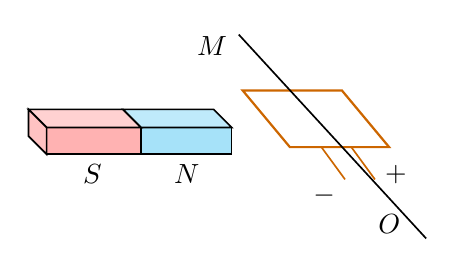
\begin{tikzpicture}[>=stealth,line width=.6pt]

\filldraw[fill=red!30](-3.2,.16)rectangle(-2,.5);
\filldraw[fill=cyan!35](-2,.16)rectangle(-.85,.5);
\filldraw[fill=red!18](-3.2,.5)--(-3.43,.73)--(-2.23,.73)--(-2,.5)--cycle;
\filldraw[fill=cyan!25](-2,.5)--(-2.23,.73)--(-1.08,.73)--(-.85,.5)--cycle;
\filldraw[fill=red!24](-3.2,.16)--(-3.43,.39)--(-3.43,.73)--(-3.2,.5)--cycle;
\node[below] at (-2.62,.16) {$S$};\node[below] at (-1.42,.16) {$N$};
\draw[orange!80!black,thick](-.71,.97)--(.55,.97)--(1.15,.25)--(-.11,.25)--cycle;
\draw[orange!80!black] (.29,.25)--(.59,-.16) (.67,.25)--(.97,-.16);
\draw(-.76,1.68)--(1.62,-.91);
\node[left]at(-.78,1.53){$M$};\node[left]at(1.42,-.73){$O$};
\node[below left]at(.59,-.12){$-$};\node[right]at(.97,-.1){$+$};

\end{tikzpicture}\end{center}
Рамку с постоянным током удерживают неподвижно в поле полосового магнита (см. рис.). Полярность подключения источника тока к выводам рамки показана на рисунке. Как будет двигаться рамка на неподвижной оси MО, если рамку не удерживать? Ответ поясните, указав, какие физические закономерности вы использовали для объяснения. Считать, что рамка испытывает небольшое сопротивление движению со стороны воздуха.
}{
\smallskip\noindent\textbf{Решение}\par
Линии магнитного поля, созданного постоянным магнитом, направлены вправо. По рамке течет ток от плюса к минусу. Выясним направление силы Ампера, с которой магнитное поле действует на каждую сторону данной рамки. В дальней от магнита стороне рамки ток течет в плоскость рисунка. По правилу левой руки сила Ампера направлена вертикально вниз. В ближней от магнита стороне рамки ток течет из плоскости рисунка. По правилу левой руки сила Ампера направлена вертикально вверх. На горизонтальные стороны рамки сила Ампера не действует, так как угол между вектором магнитной индукции и направлением тока равен $0^\circ$ или $180^\circ$, для которых  $\sin \alpha = 0$  и сила Ампера $F_A=BIl \sin \alpha =0.$
В результате действия противоположно направленных сил на стороны рамки она будет поворачиваться по часовой стрелке, двигаясь замедленно из-за сопротивления воздуха. Кроме того, при повороте рамки на угол чуть больший $90^\circ$ силы Ампера будут рамку тормозить. В результате рамка расположится вертикально, ее плоскость будет перпендикулярна магнитным линиям.
}

\end{document}
